% !TEX root = CartaPerali_Report.tex
\section{Processing Pipeline}
\label{sec:processing_pipeine}

\noindent The code necessary to replicate this work is available in the GitHub repository \footnote{https://github.com/Fisher4537/HumanDataAnalitycs}.\\
The workflow used to implement the whole KWS system is depicted in Fig. \ref{fig:pipeline}.
\begin{figure}[h]
			\centering
	    	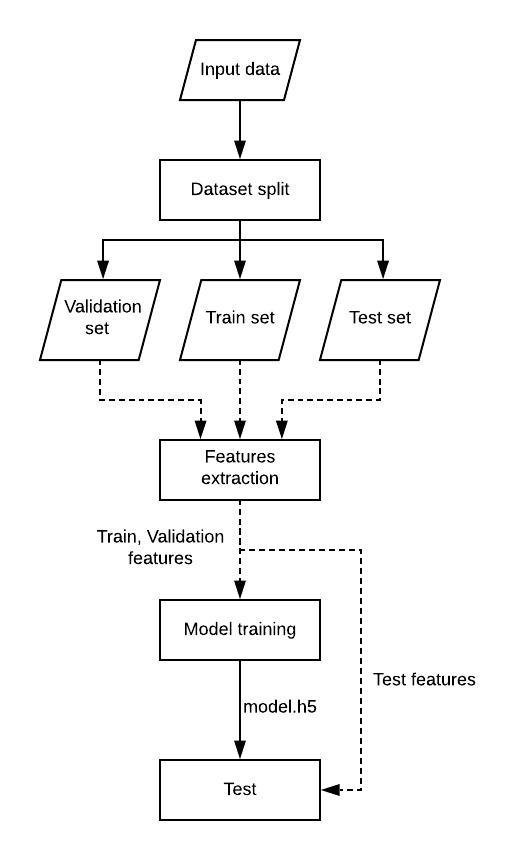
\includegraphics[width=6cm, height=8cm ,width=0.25\textwidth]{pipeline}
	    	\caption{System workflow}
	    	\label{fig:pipeline}
\end{figure} 
\noindent As mentioned in the intro, the input data are downloaded from the well known public '{\it{speech\_commands V2}}' dataset \cite{Warden-2018}. At the time of this project it counts 105829 audio file, in \textit{.wav} format, 16000 Hz, channel mono with the duration of one second each. Each of them is listed and the file dimension is checked: only the file with size of 32K are kept, the other are discarded, indeed the audio with length less than 1 s have an higher probability to contain truncated word spell. \\
As suggested by the author of the dataset \cite{Warden-2018}, to split the it into \textit{train}, \textit{validation} and \textit{test}, the hash of each audio is used to avoid that two different audio with the same label and pronounced by the same person would be put on different set (see \textit{which\_set} method described by the author in the README), compromising the interdependence between the different sets. \\
The dataset is too huge be loaded into conventional RAM, therefore each list (train, validation and test) is dynamically split into lighter batches by specific generator (represented as dashed line in fig. \ref{fig:pipeline}). Each generator return a preprocessed audio as described next, which is consumed during the train and/or test phase.\\ \\
\textbf{Balanced batches and unknown percentage.} In a real application an audio stream is full of background noise and utterance to ignore. The keywords to recognize are only a little part. To differentiate background noise and unknown utterance, an \textit{unknown} label is added to the wanted words. The \textit{unknown} class should be composed of audio depending of the application context. In this report the problem is not faced. However it is provided a simple mechanism for the management of unknown label and the percentage of each label of the dataset. A list of \textit{wanted words} is passed as input parameter with an unknown percentage value. Each returned batch has the specified percentage of unknown audios taken from the file which are not in the wanted word list. In the report, each dataset with a specific percentage of unknown is defined as \textit{balanced}, instead, \textit{unbalanced} dataset has no specific unknown percentage and that class composed of all the speech recognition audio that are not labeled with a specified wanted word.


\section{Data preprocessing and Features extraction}
\label{sec:model}

\noindent Data are preprocessed by \textit{generators} that are responsible for preparing batches of data containing the desired percentage of predefined wanted words, organized in a list and the percentage of words that the model should classify as \textit{unknown} if used.\\
The preprocessed example are obtained from the raw signal of the "bad" utterance represented in figure \ref{fig:bed_rawsignal}.\\

\noindent \textbf{MFCC.} The raw data is normalized from -1 to 1 and the Mel-Frequency Cepstrum Coefficients are computed with \textit{python\_speech\_features} library. This one apply the Fast Fourier Transform, the power of the spectrum obtained is mapped onto the mel scale using triangular overlapping, then the logs of the powers at each of the mel frequencies is taken and in the end the discrete cosine transform of the list of mel log powers is computed. MFCC frames are built using the selected parameters depicted in Table \ref{table:mfcc_parameters}.
\noindent In the end, one set of 13 MFCC coefficients is extracted from each frame. In figure \ref{fig:bed_mfcc} is shown an example of preprocess of an input signal.
\begin{table}[h]
	\centering
	\begin{tabular}{ |l|c|}
		\hline
		Window length & 25 ms        \\
		Window step & 0.01 ms        \\
		Frame shift  & 10 ms         \\
		N. of coefficients & 13 \\
		N. Filterbanks & 26         \\
		N. FFT points & 512         \\
		\hline
	\end{tabular}
	\caption{MFCC parameters}
	\label{table:mfcc_parameters} 
\end{table}\\
\noindent \textbf{Spectrogram.} Raw data are normalized from 1 to -1, split into segments, multiply by the windowing function and then the Fast Fourier Transform is apply.
The parameter values used to compute the spectrogram are in Table \ref{table:specgram_parameters}. In figure \ref{fig:bed_specgram} is shown an example of preprocess of an input signal.
\begin{table}[h]
	\centering
	\begin{tabular}{ |l|c| }
		\hline
		N. of points per segment & 256 \\
		Windowing function & Hanning window \\
		N. of overlapping points between segments & 128 \\
		\hline
	\end{tabular}
	\caption{Spectrogram parameters}
	\label{table:specgram_parameters} 
\end{table}\\

\begin{figure}
	\centering
	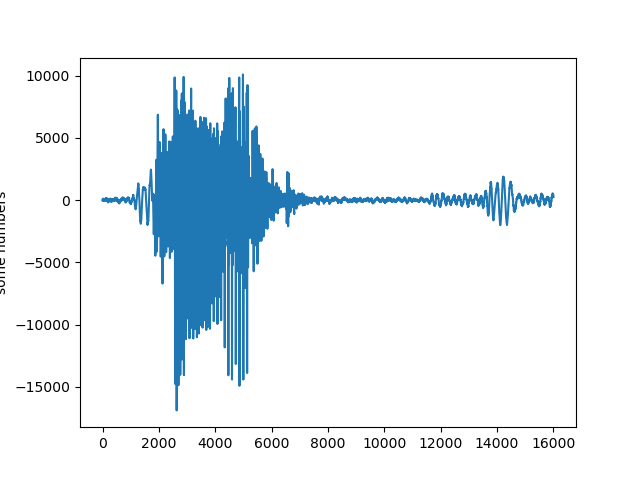
\includegraphics[width=.5\textwidth]{img/bed_rawsignal_plot.png}
	\caption{Raw signal of the \textit{bad} utterance}
	\label{fig:bed_rawsignal}
\end{figure}


\begin{figure}
	\centering
	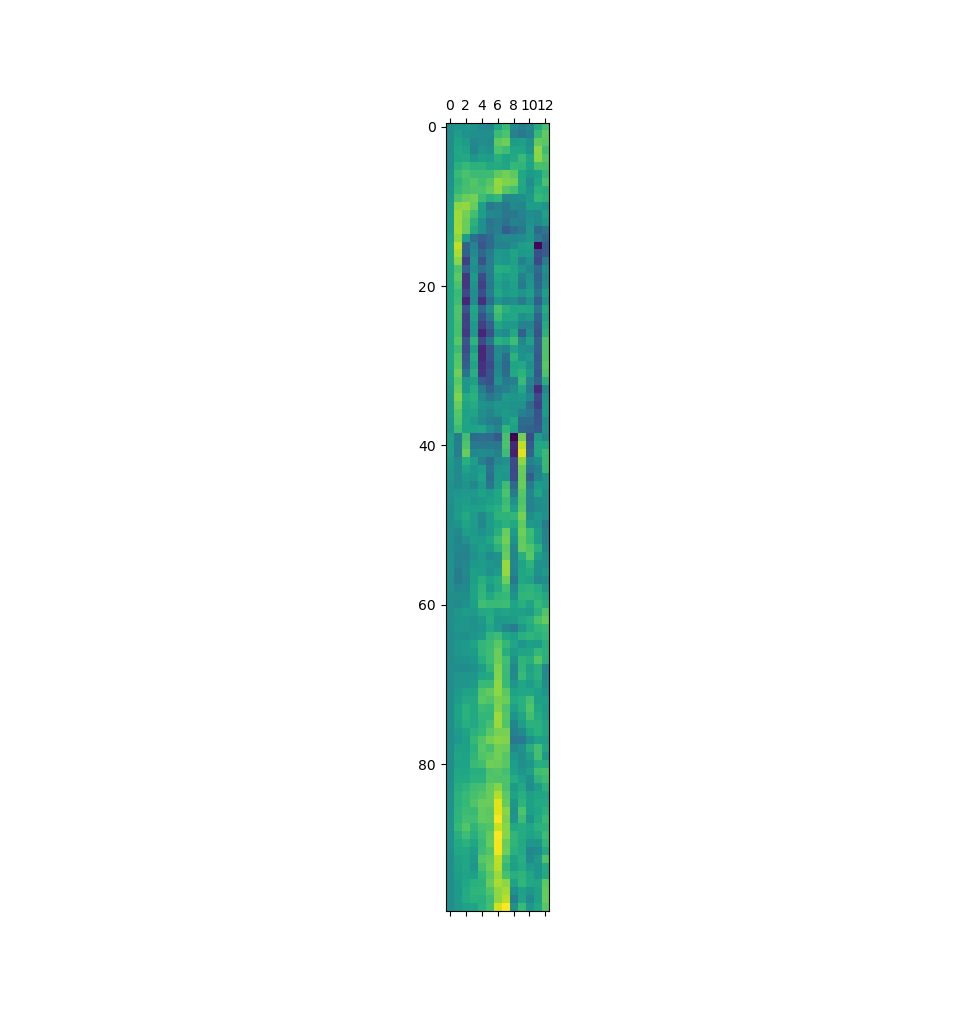
\includegraphics[width=0.5\textwidth]{img/bed_mfcc_plot.png}
	\caption{MFCC of the \textit{bad} utterance}
	\label{fig:bed_mfcc}
\end{figure}


\begin{figure}
	\centering
	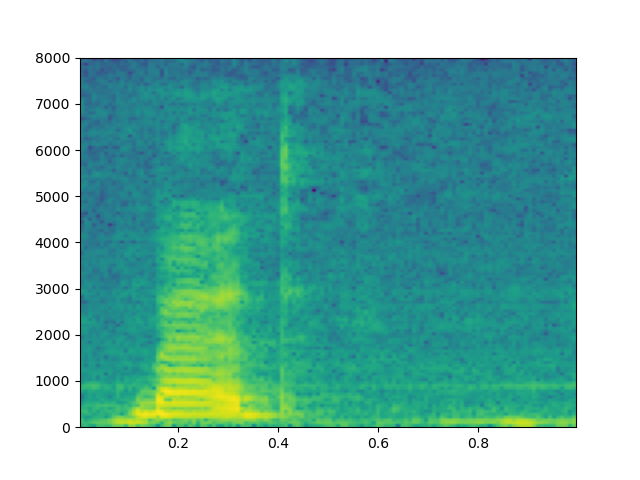
\includegraphics[width=0.5\textwidth]{img/bed_specgram_matplotlib.png}
	\caption{Spectrogram of the \textit{bad} utterance}
	\label{fig:bed_specgram}
\end{figure}


\section{Learning Framework}
\label{sec:learning_framework}

\subsection*{\textbf {CNN architecture}}
\label{subsec:arch}
\noindent Processed input data contain at this point the feature vectors ready to be fed as input to the model. Different CNN architechtures have been tested. The types of layer composing the final CNN architechture are the following:
\begin{itemize}
\item {\it{Convolutional layer}}: responsible of learning the features. In this type of layer, regularization is applied to prevent overfitting.
\item {\it{Pooling layer}}: performs down-sampling by taking max operation. This reduces the amount of parameters in the network, and hence controls overfitting.
\item {\it{Flattern layer}}: flattens the input. It's placed between a convolutional and a dense layer.
\item {\it{Dense layer}}: also known as fully-connected layer, receives the input from convolutional layers or can be the last layer in the network, thus used to make a softmax prediction.
\item {\it{Dropout layer}}: placed between two subsequent fully-connected layers, ignore some neurons with a certain probability during the training phase. It is used to prevent overfitting.\\

\noindent The layers described above, are combined to build the desired CNN architecture as shown in Fig. \ref{fig:CNN_schema}.  

\end{itemize}
\begin{figure}[ht]
	\centering
	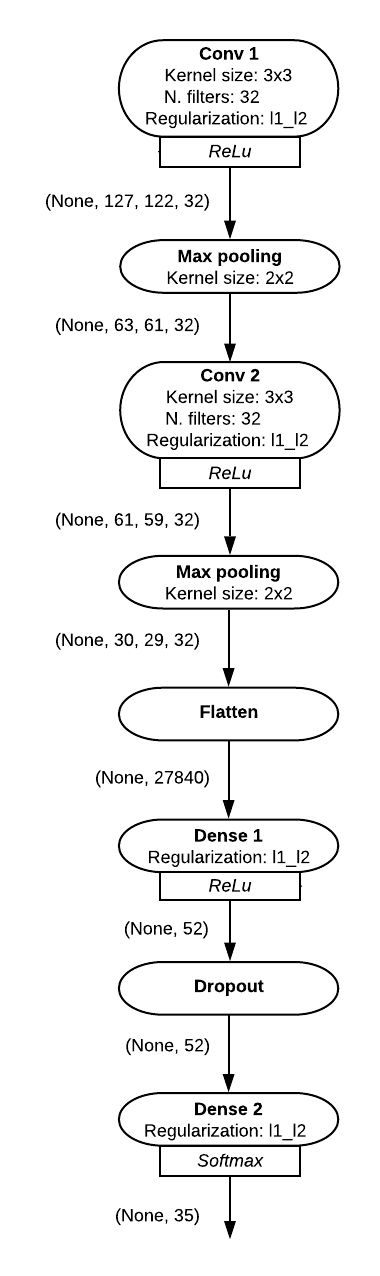
\includegraphics[scale=0.6]{CNN_schema}
	\caption{CNN schema}
	\label{fig:CNN_schema}
\end{figure} 

\section{Training analysis}
\noindent The training phase of the model described in Section. \ref{sec:learning_framework} was conducted on different amounts of epochs combined with different learning rates to achieve the beste performance in terms of accuracy without overfitting.\\

\noindent \textbf{Loss function.} The {\it{categorical\_crossentropy}} was the choice for the loss function deployed in the training phase.\\

\noindent \textbf{Metric.} The {\it{accuracy}} was used to measure the behaviour of the model in the training phase.\\

\noindent \textbf{Optimizers.} Two optimizers were tested in order to subsequently compare the obtained results. The deployed optimizers are the classic {\it{Stochastic Gradient Descent}} (SGD) and the {\it{Adam}} algorithm. The former seemed to be outperformed by the latter, thus making of Adam optimizer the final choice for the training phase of the deployed CNN. Several tests were conducted to determine the best learning rate, leading to the best performance later in the test phase. \\

\noindent \textbf{Callbacks.} During the training phase of the model, several callbacks are passed as input to improve the performances in a computationally smart way:
\begin{itemize}
\item {\it{ReduceOnPlateau}}: takes care of setting the learning rate according to the behavior of the accuracy's curve.
\item {\it{EarlyStopping}}: has the purpose of stopping the training process, if no significant improvement is observed for a defined number of epochs.
\item {\it{TensorBoard}}: provides an interface to show the behavior of the metrics of interest during the training.\\
\end{itemize}

\noindent In Fig. \ref{fig:CNN_loss} the behavior of the loss during the training phase is shown and in Fig.  \ref{fig:CNN_accuracy} accuracy's one is depicted. In both pictures, the blue curve represent the validation's behaviour and the orange curve the training's one.\\The proposed model was trained for 100 epochs and from both pictures can be observed how the training process was concluded earlier by mean of the {\it{early stopping}} callback function.

\begin{figure}[h]
			\centering
	    	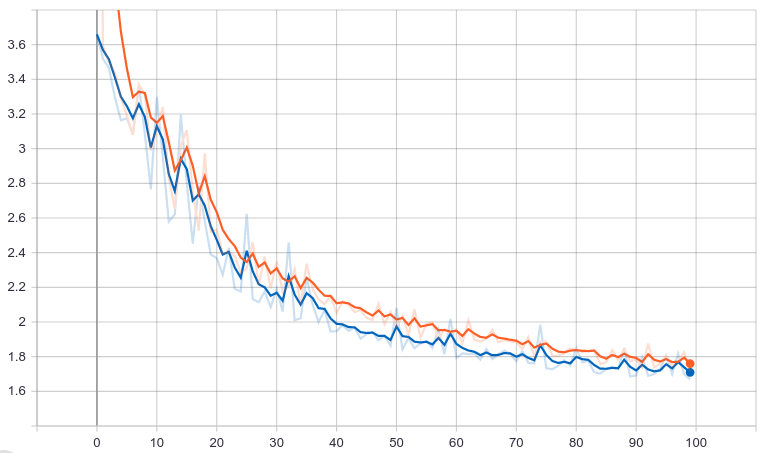
\includegraphics[width=8cm, height=6cm]{debug_tuy_loss}
	    	\caption{Training loss}
	    	\label{fig:CNN_loss}
\end{figure} 

\begin{figure}[h]
			\centering
	    	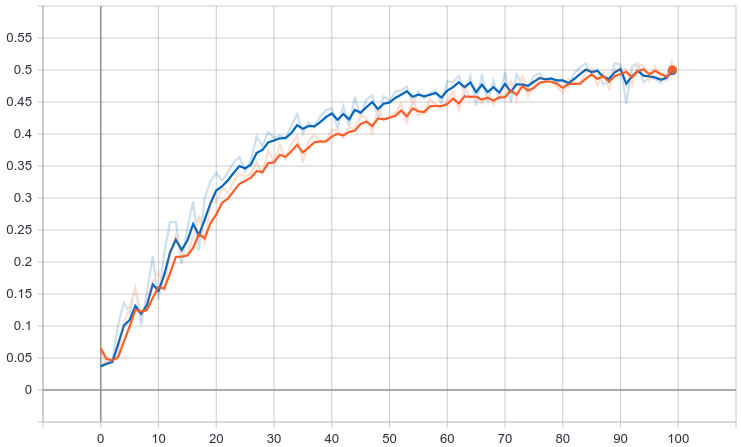
\includegraphics[width=8cm, height=6cm]{debug_tuy_acc}
	    	\caption{Training accuracy}
	    	\label{fig:CNN_accuracy}
\end{figure} 

\noindent In Table. \ref{table:CNN_parameters} a summary of the number of parameters of the trained CNN model.\\

\begin{table}[h!]
\centering
\begin{tabular}{| l | c |}
\hline
Total params &1,459,155\\
Trainable params& 1,459,155\\
Non-trainable params& 0\\
\hline
\end{tabular}
\caption{CNN parameters}
\label{table:CNN_parameters}
\end{table}




